\documentclass[xcolor=dvipsnames,table]{beamer}

\usepackage{latexsym}
\usepackage[utf8]{inputenc}
\usepackage[brazil]{babel}
\usepackage{amssymb}
\usepackage{amsmath}
\usepackage{stmaryrd}
\usepackage{fancybox}
\usepackage{datetime}
\usepackage[T1]{fontenc}
\usepackage{graphicx}
\usepackage{graphics}
\usepackage{url}
\usepackage{algorithmic}
\usepackage{algorithm}
\usepackage{acronym}
\usepackage{array}

\newtheorem{definicao}{Definio}
\newcommand{\tab}{\hspace*{2em}}

\mode<presentation>
{
  \definecolor{colortexto}{RGB}{0,0,0}
 
  \setbeamertemplate{background canvas}[vertical shading][ bottom=white!10,top=white!10]
  \setbeamercolor{normal text}{fg=colortexto} 

  \usetheme{Warsaw}
}

\title{Decidibilidade} 

\author{
  Esdras Lins Bispo Jr. \\ \url{bispojr@ufg.br}
  } 
 \institute{
  Teoria da Computação \\Bacharelado em Ciência da Computação}
\date{\textbf{29 de junho de 2017} }

\logo{
\includegraphics[width=1cm]{images/ufgJataiLogo.png}}

\begin{document}

	\begin{frame}
		\titlepage
	\end{frame}

	\AtBeginSection{
		\begin{frame}{Sumário}%[allowframebreaks]{Sumário}
    		\tableofcontents[currentsection]
    		%\tableofcontents[currentsection, hideothersubsections]
		\end{frame}
	}

	\begin{frame}{Plano de Aula}
		\tableofcontents
		%\tableofcontents[hideallsubsections]
	\end{frame}
    
    \section{Revisão}
    
	\subsection{Decidibilidade}
	
	\begin{frame}{Problema da Igualdade de Linguagens}
		\begin{block}{Descrição}
			Dadas duas linguagem $L_1$ e $L_2$, identificar se $L_1 = L_2$.
		\end{block}	 
		\begin{block}{Problema aplicado a AFDs}
			$EQ_{AFD} = \{ \langle A, B \rangle \mbox{ | } A$ e $B$ são AFDs e $L(A) = L(B) \}$
		\end{block}  
		\begin{block}{Estratégia de Resolução}
			Decidir se $\langle A, B \rangle \in EQ_{AFD}$.
		\end{block}
	\end{frame}		
	
	\begin{frame}{Problema da Igualdade de Linguagens}
		\begin{block}{Teorema 4.5}
			$EQ_{AFD}$ é uma linguagem decidível.
		\end{block}  
		\begin{block}{Lema 4.1}
			Iremos construir um AFD $C$ a partir de $A$ e $B$ de forma que $C$ aceita as cadeias que são aceitas por $A$ ou por $B$, mas não por ambas. Consequentemente, se $A$ e $B$ reconhecem a mesma linguagem, $C$ não aceitará nada. A linguagem de $C$ é
			\begin{center}
				$L(C) = \left( L(A) \cap \overline{L(B)} \right) \cup \left( \overline{L(A)} \cap L(B) \right)$
			\end{center}
		\end{block}  
		\begin{block}{Corolário}
			$L(C) = \emptyset$ \ $\leftrightarrow$ \ $L(A) = L(B)$
		\end{block}
	\end{frame}
	
	\begin{frame}{Problema da Igualdade de Linguagens}
		\begin{center}
			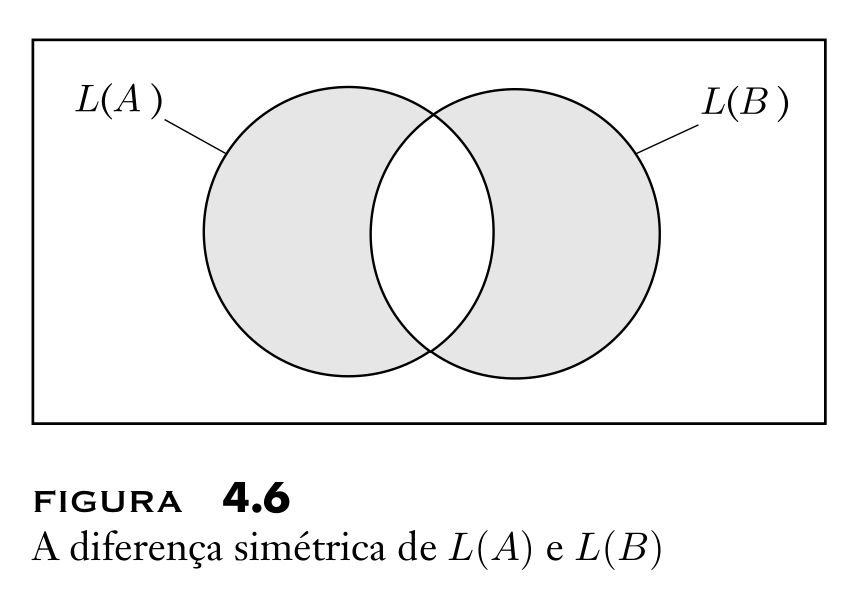
\includegraphics[width=9cm]{images/fig46.png}
		\end{center}
	\end{frame}
	
	\begin{frame}{Problema da Igualdade de Linguagens}
		\begin{block}{Teorema 4.5}
			$EQ_{AFD}$ é uma linguagem decidível.
		\end{block}  
		\begin{block}{Prova}
			A seguinte MT $F$ decide $EQ_{AFD}$.
			
			$F$ = ``Sobre a entrada $\langle A, B \rangle$, em que $A$ e $B$ são AFDs:
			\begin{enumerate}
				\item Construa o AFD $C$ conforme descrito no Lema 4.1;
				\item Rode MT $T$ do Teorema 4.4 sobre a entrada $\langle C \rangle$;
				\item Se $T$ aceita, {\bf aceite}. Caso contrário, {\bf rejeite}.''
			\end{enumerate}
		\end{block}
	\end{frame}
	
	\begin{frame}{Teoremas sobre GLC}
		\begin{block}{Teorema 4.7}
			$A_{GLC}$ é uma linguagem decidível.
		\end{block}
		\begin{block}{Teorema 4.8}
			$V_{GLC}$ é uma linguagem decidível.
		\end{block}
		\begin{block}{Teorema 4.9}
			Toda LLC é decidível.
		\end{block}  
		\begin{alertblock}{Cuidado!}
			$EQ_{GLC}$ {\color{red} {\bf não}} é uma linguagem decidível.
		\end{alertblock}
	\end{frame}
	
	\begin{frame}{Relacionamento entre as classes de linguagens}
		\begin{center}
			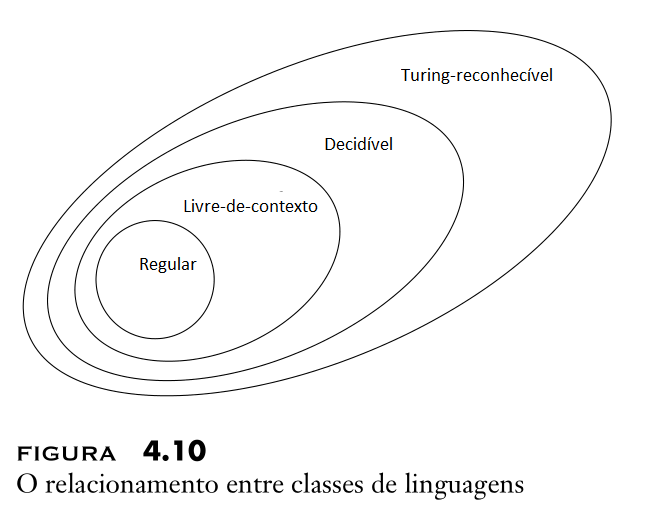
\includegraphics[width=9cm]{images/fig410.png}
		\end{center}
	\end{frame}
	
	\subsection{O Problema da Parada}
	\begin{frame}{O Problema da Parada}
		\begin{block}{Problema da aceitação para MT}
			Dada uma MT $M$ e uma cadeia de entrada $\omega$, identificar se $M$ aceita $\omega$.
		\end{block}	 
		\begin{block}{Problema}
			$A_{MT} = \{ \langle M, \omega \rangle$  | $M$ é uma MT que aceita a cadeia de entrada $\omega \}$
		\end{block}  
		\begin{alertblock}{Teorema 4.11}
			$A_{MT}$ é indecidível.
		\end{alertblock}
	\end{frame}
	
	\begin{frame}{O Problema da Parada}
		\begin{block}{Considerações sobre o Teorema 4.11}
			$A_{MT}$ é Turing-reconhecível. Pois é possível construir $U$ da seguinte forma:  
			
			$U$ = ``Sobre a entrada $\langle M, \omega \rangle$, em que $M$ é uma MT e $\omega$ uma cadeia:
			\begin{enumerate}
				\item Simule $M$ sobre a entrada $\omega$;
				\item Se $M$ em algum momento entra no seu estado de aceitação, {\bf aceite}; se $M$ em algum momento entra em seu estado de rejeição, {\bf rejeite}.''
			\end{enumerate}
		\end{block}	 
		\begin{alertblock}{Problema da Parada}
			Não é possível construir uma MT que decida $A_{MT}$.
		\end{alertblock} 
	\end{frame}
	
	\begin{frame}{O Problema da Parada}
		\begin{block}{Máquina de Turing Universal}
			É uma MT capaz de simular qualquer outra MT. \\A MT $U$ apresentada anteriormente é uma MT Universal.
		\end{block}  
		\begin{exampleblock}{Contribuição importante}
			A MT Universal estimulou o desenvolvimento de computadores com programas armazenado.
		\end{exampleblock} 
	\end{frame}
	
	\begin{frame}{O Problema da Parada}
		\begin{center}
			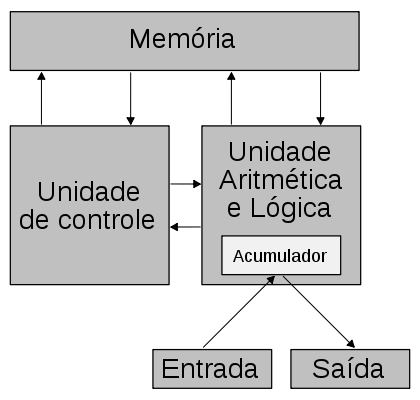
\includegraphics[width=6cm]{images/arqVonNeumann.png}
			
			{\bf Figura:} Arquitetura de von Neumann (1945).
		\end{center}
	\end{frame}
	
	\begin{frame}{Método da diagonalização}
		\begin{columns}
			\column{.4\textwidth}  		
			\begin{center}
				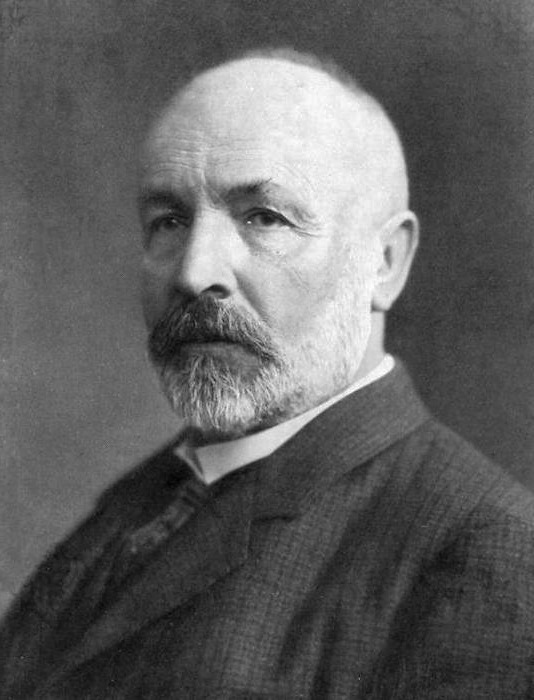
\includegraphics[height=.6\textheight]{images/cantor.jpg}
			\end{center}
			\column{.6\textwidth}  		
			\begin{block}{Contribuição}
				\begin{center}
					{\large Criou o método da diagonalização em 1873.}
				\end{center}
			\end{block}		  		
			\begin{block}{Quem?}
				\begin{center}
					{\bf George Cantor (1845-1918)} \\ Matemático russo.
				\end{center}
			\end{block}
		\end{columns}
	\end{frame}
	
	\begin{frame}{Método da diagonalização}
		\begin{alertblock}{Problema}
			Se temos dois conjuntos infinitos, como podemos dizer se um conjunto é maior que o outro (ou se eles têm o mesmo tamanho)?
		\end{alertblock}  
		\begin{block}{Conjuntos finitos}
			Podemos utilizar o método da contagem.
		\end{block}  
		\begin{exampleblock}{Proposta de Cantor}
			Dois conjuntos finitos têm o mesmo tamanho se os elementos de um deles puder ser emparelhados com os elementos do outro. Basta estendermos essa ideia para os conjuntos infinitos!
		\end{exampleblock}
	\end{frame}

	\section{Método da diagonalização}
	
	\begin{frame}{Método da diagonalização}
		\begin{block}{Função um-para-um}
			Sejam dois conjuntos $A$ e $B$ e uma função $f$ de $A$ para $B$. Dizemos que $f$ é {\bf um-para-um} se ela nunca mapeia dois elementos diferentes para um mesmo lugar (ou seja, $f(a) \not= f(b)$ sempre que $a \not= b$).
		\end{block}	\pause	
		\begin{block}{Função Sobrejetora}		
			Uma função $f$ é {\bf sobrejetora} se ela atinge todo elemento de $B$ \\(ou seja, se para todo $b \in B$ existir um $a \in A$ tal que $f(a) = b$).
		\end{block} 
	\end{frame}
	
	\begin{frame}{Método da diagonalização}
		\begin{block}{Correspondência}
			Uma {\bf correspondência} é uma função que é tanto um-para-um, quanto sobrejetora. Em uma correspondência $f : A \rightarrow B$, todo elemento de $A$ é mapeado para um único elemento de $B$ e cada elemento de $B$ tem um único elemento de $A$ mapeando para ele. 
		\end{block} \pause
		\begin{block}{Tamanho de conjuntos}
			Dois conjuntos $A$ e $B$ são de {\bf mesmo tamanho} se existe uma correspondência de $A$ para $B$.
		\end{block}
	\end{frame}
	
	\begin{frame}{Método da diagonalização}
		\begin{block}{Exemplo 1}
			\begin{itemize}
				\item $\mathbb{N} = \{ 1, 2, 3, ... \}$
				\item $P = \{ x$ | $x$ é par $\}$
			\end{itemize} 
		\end{block} \pause
		\begin{block}{$\mathbb{N}$ e $P$ têm o mesmo tamanho} \pause
			\begin{itemize}
				\item É possível encontrar uma correspondência entre $\mathbb{N}$ e $P$; \pause
				\item $f:\mathbb{N} \rightarrow P$ em que $f(n) = 2n$;
			\end{itemize}
		\end{block}	
	\end{frame}
	
	\begin{frame}{Método da diagonalização}
		\begin{center}
			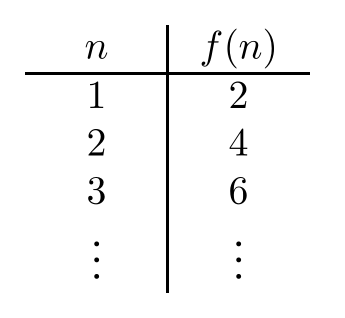
\includegraphics[width=6cm]{images/fn2n.png}
			
			{\bf Figura:} Visualização de $f$ através de uma tabela.
		\end{center}
	\end{frame}
	
	\begin{frame}{Método da diagonalização}
		\begin{block}{Considerações}
			\begin{itemize}
				\item Pode parecer contra-intuitivo, pois $P \subseteq \mathbb{N}$; \pause
				\item Mas é possível fazer a correspondência entre os conjuntos; \pause
				\item Logo, declaramos que esses conjuntos têm o mesmo tamanho.			
			\end{itemize}
		\end{block} \pause
		\begin{block}{Conjunto Contável}
			Um conjunto $A$ é {\bf contável} se é finito ou \\se tem o mesmo tamanho de $\mathbb{N}$.
		\end{block}
	\end{frame}
	
	\begin{frame}{Método da diagonalização}
		\begin{block}{Exemplo 2}
			Seja $\mathcal{Q} = \{ m / n$ | $m, n \in \mathbb{N} \}$ o conjunto dos racionais positivos.
		\end{block} \pause
		\begin{block}{$\mathcal{Q}$ é contável (curiosamente)} 
			Logo $\mathcal{Q}$ é finito ou tem o mesmo tamanho de $\mathbb{N}$.
		\end{block}
	\end{frame}
	
	\begin{frame}{Método da diagonalização}
		\begin{center}
			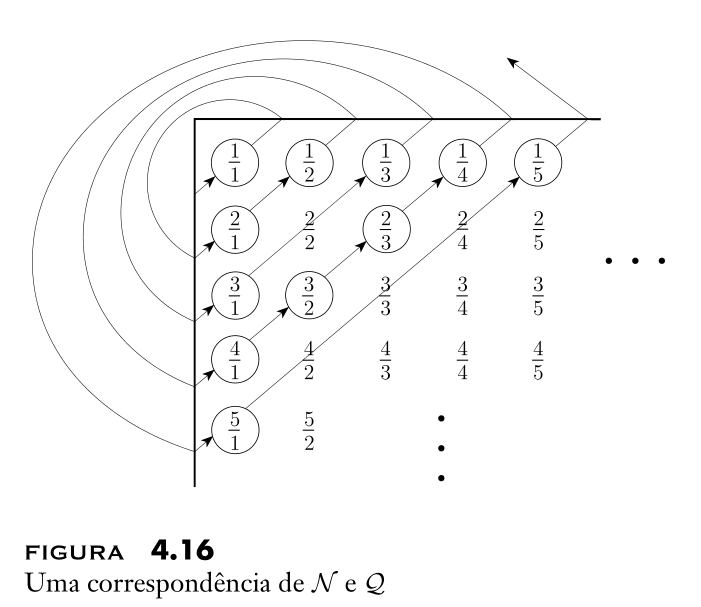
\includegraphics[width=8cm]{images/diagonal.png}
		\end{center}
	\end{frame}
	
	\begin{frame}{Método da diagonalização}
		\begin{block}{Considerações}
			\begin{itemize}
				\item Ao ver o exemplo de  $\mathcal{Q}$, há uma ligeira impressão de que qualquer conjunto é contável; \pause
				\item Mas existe conjuntos incontáveis; \pause
				\item Cantor provou que $\mathbb{R}$ é incontável introduzindo o \\método da diagonalização.
			\end{itemize}
		\end{block} \pause
		\begin{block}{Teorema 4.17}
			$\mathbb{R}$ é incontável.
		\end{block}
	\end{frame}

	\begin{frame}
		\titlepage
	\end{frame}
	
\end{document}